\chapter{Topological Space}\label{1_1}

This chapter opens with the definition of a topology and 
is then devoted to some simple examples.
\par
Topology, like other branches of pure mathematics such group theory,
is an axiomatic subjece. We start with a set of axioms and we use these 
axioms and we use these axioms to prove propositions and theorems. 
It is extremely important to develop your skill at writing proofs.
\section{Topological Space}
\begin{definition}{}{}
    Let $X$ be a non-empty set. A set $\tau\subseteq \mathcal{P}(X)$ is said to be 
    a topology on $\mathcal{X}$ if\\
    (1) $X,\O\in\tau$, \\
    (2) If $U_{\alpha}\in\tau$($\alpha\in I$, $I$ is finite or infinite), then $\cup_{\alpha\in I}U_{\alpha}\in \tau$,\\
    (3) If $U_1,U_2\in \tau$, then $U_1\cap U_2\in \tau$. 
\end{definition}

\begin{example}{Trivial topology}{}
        Let $X$ be any non-empty set and $\tau_t = \{X,\O\}$.
        Then $\tau_t$ is called the trival topology on $X$. 
\end{example}
(1) $X,\O\in\tau$;\   (2) $X\cup \O=X\in\tau$;\  (3) $X\cap\O=\O\in\tau$.

\begin{example}{Discrete topology}{}
    Let $X$ be any non-empty set and $\tau_s = \mathcal{P}(X)$.
        Then $\tau_s$ is called the discrete topology on $X$.
\end{example}
(1) $X,\O\in\tau$;\   (2) $\cup U_{\alpha}\in\tau$;\  (3) $U_1\cap U_2\in\tau$.

\begin{example}{Cofinite topology}{}
    Let $X$ be any non-empty set and $\tau_f = \{U\subseteq X: U=\O \ or \ U^{c}\ is \ finite\}$.
        Then $\tau_f$ is called the cofinite topology on $X$.
\end{example}
(1) $\O\in\tau$, $X^c=\O$ is finite with cardinality zero, then $X\in\tau$;
\par
(2) If $U_{\alpha}\in\tau$ and $U_{\alpha}\neq\O$ ($\O$ has no effect on union).
Let $U=\cup U_{\alpha}$, then $U^c=\cap U_{\alpha}^c$ is the intersection of finite set and so $U^c$ is finite.
Hence, $U\in\tau$;
\par
(3) If $U_1,U_2\in\tau$, let $U=U_1\cap U_2$. Then $U^c=U_1^c\cup U_2^c$ is the union of finite set and so $U^c$ is finite.
Hence, $U\in\tau$. 

\begin{example}{Cocountable topology}{}
    Let $X$ be any non-empty set and $\tau_c = \{U\subseteq X: U=\O \ or \ U^{c}\ is \ countable\}$.
        Then $\tau_c$ is called the cocountable topology on $X$.
\end{example}
(1) $\O\in\tau$, $X^c=\O$ is finite with cardinality zero, then $X\in\tau$;
\par
(2) If $U_{\alpha}\in\tau$ and $U_{\alpha}\neq\O$ ($\O$ has no effect on union).
Let $U=\cup U_{\alpha}$, then $U^c=\cap U_{\alpha}^c$ is the intersection of countable set and so $U^c$ is countable.
Hence, $U\in\tau$;
\par
(3) If $U_1,U_2\in\tau$, let $U=U_1\cap U_2$. Then $U^c=U_1^c\cup U_2^c$ is the union of countable set and so $U^c$ is countable.
Hence, $U\in\tau$. 

\begin{example}{Euclidean topology}{}
    $\tau_e = \{U : U=\cup_{(a,b)\in I} (a,b), a<b\in \R, I \text{ is a collection of open interval}\}$. $I$ can be infinite, finite or zero.
        Then $\tau_e$ is called the euclidean topology on $\R$. We write $E^1=(\R,\tau_e)$.
\end{example}
(1) $\O$ = empty union. Then $\O\in \tau$. 
For every $x\in \R$, there exists $(a_x,b_x)$ s.t. $x\in(a_x,b_x)$, 
then $\R=\cup_{x\in\R}(a_x,b_x)\in\tau$.
\par
(2) (3) refer to topology without tears page 51.

\section{Metric Topology}

The most important class of topological spaces is the class of metric spaces.
Metric spaces provide a rich source of examples in topology. But more than this, 
most of the applications of topology to analysis are via metirc spaces.

\begin{definition}{}{}
    Let $X$ be a non-empty set and $d$ a real-valued function defined on $X\times X$ such that for $x,y,z\in X$:
    \\
    (1) $d(x,y)\geqs 0$ and $d(x,y)=0$ iff $x=y$;\\
    (2) $d(x,y)=d(x,y)$;\\
    (3) $d(x,z)\leqs d(x,y) + d(y,z)$.\\
    Then $d$ is said to be a metric on $X$, $(X,d)$ is called a metric space and $d(a,b)$ is referred to as the distance between $a$ and $b$.
\end{definition}

\begin{example}{}{}
    $\R^n=\{(x_1,x_2,...,x_n)|x_i\in \R,i=1,2,...,n\}$. We defined the metirc in $\R^n$ as
    \begin{align*}
        d((x_1,...,x_n),(y_1,...,y_n)) = \sqrt{\sum\limits_{i=1}^{n}(x_i-y_i)^2}, 
    \end{align*}
    $(\R^n,d)$ is called $n$ dimension euclidean space, denoted by $E^n$.
\end{example}

\begin{definition}{}{}
    Let $(X,d)$ be a metirc space and $\epsilon$ any positive real number. Then the open ball about $x_0\in X$ of radius $\epsilon$ is the set
    $B(x_0,\epsilon)=\{x\in X:d(x_0,x)\leq\epsilon\}$
\end{definition}

\begin{example}{}{}
    In $\R$ with the euclidean metric, $B(x_0,\epsilon)$ is the open interval $(x_0-\epsilon, x_0+\epsilon)$.
\end{example}

\begin{lemma}{}{open ball intersection point}
    Let $(X,d)$ be a metric space and $x,y\in X$.
    Further, let $\epsilon_1$ and $\epsilon_2$ be positive real numbers. 
    If $z\in B(x,\epsilon_1)\cap B(y,\epsilon_2)$, 
    then there exists a $\epsilon>0$ such that $B(z,\epsilon)\subseteq B(x,\epsilon_1)\cap B(y,\epsilon_2)$.
\end{lemma}

\begin{proof}
    Let $\epsilon = \min\{\epsilon_1-d(x,z),\epsilon_2-d(y,z)\}$, then for $a\in B(z,\epsilon)$,
    \begin{align*}
        d(a,x)&\leqs d(a,z)+d(z,x)\leqs \epsilon + d(x,z)= \epsilon_1,\\
        d(a,y)&\leqs d(a,z)+d(z,y)\leqs \epsilon + d(y,z)= \epsilon_2.
    \end{align*}
    Hence, $a\in B(x,\epsilon_1)\cap B(y,\epsilon_2)$ and so $B(z,\epsilon)\subseteq B(x,\epsilon_1)\cap B(y,\epsilon_2)$.
\end{proof}

\begin{corollary}{}{open ball intersection union}
    Let $(X,d)$ be a metric space and $B_1$ and $B_2$ open balls in $(X,d)$. Then
    $B_1\cap B_2$ is a union of open balls in $(X,d)$.
\end{corollary}
\begin{proof}
    By lemma\ref{lem:open ball intersection point}, $\forall z\in B_1\cap B_2$, 
    there exists $\epsilon_z>0$ such that $B(z,\epsilon_z)\subseteq B_1\cap B_2$. Then
    $\cup_{z\in B_1\cap B_2} B(z,\epsilon_{z})\subseteq B_1\cap B_2\subseteq \cup_{z\in B_1\cap B_2} B(z,\epsilon_{z})$. 
    Hence, $B_1\cap B_2 = \cup_{z\in B_1\cap B_2} B(z,\epsilon_{z})$
\end{proof}


\begin{proposition}{}{}
    Let $(X,d)$ be a metric space. Then $\tau_d=\{U: U=\cup_{\alpha} B(x_{\alpha}, \epsilon_{\alpha}) \}$ is a topology on $X$. 
\end{proposition}
\begin{proof}
    (1) $\O$ = empty union, then $\O\in \tau_d$. $X=\cup_{x\in X}B(x,\epsilon_{x})\in \tau_d$.\\
    (2) The union of open ball union is open ball union.\\
    (3) If $U,U'\in \tau_d$, then $U=\cup_{\alpha} B(x_{\alpha}, \epsilon_{\alpha})$, $U'=\cup_{\beta} B(x_{\beta}, \epsilon_{\beta})$, then
    \begin{align*}
        U\cap U' &= (\cup_{\alpha} B(x_{\alpha}, \epsilon_{\alpha}))\cap(\cup_{\beta} B(x_{\beta}, \epsilon_{\beta}))\\
                &= \cup_{\alpha,\beta} (B(x_{\alpha}, \epsilon_{\alpha})\cap B(x_{\beta}, \epsilon_{\beta})).
    \end{align*}
    By corollary\ref{cor:open ball intersection union}, $B(x_{\alpha}, \epsilon_{\alpha})\cap B(x_{\beta}, \epsilon_{\beta})$ is the union of open ball. 
    Then $U\cap U'$ is the union of open ball.
\end{proof}

$\tau_d$ is called the topology induced by metirc or simply metric topology. 

\section{Basic Conception in Topological Space}

Rather than continually refer to "members of $\tau$", we find it more convenient to give such sets a name. 
We call them "open sets". We shall also name the complements of open sets. They will be called "closed sets". 

\subsection{Open set}
\begin{definition}{}{}
    Let $(X,\tau)$ be any topological space. Then the members of $\tau$ are said to be open sets.
\end{definition}

\begin{proposition}{}{open set judging}
    Let $U$ be a subset of a topological space $(X,\tau)$.
    Then $U\in\tau$ iff for each $x\in U$ there exists $U_x\in\tau$ such that $x\in U_x\subseteq U$.
\end{proposition}
\begin{proof}
    ($\Rightarrow$): Since $U\in\tau$, for each $x\in U$, take $K=U$, then $x\in K\subseteq U$.\\
    ($\Leftarrow$): Since $U\subseteq \cup_{x\in U}U_x\subseteq U$, $U=\cup_{x\in U}U_x\in\tau$. 
\end{proof}
\begin{remark}
    This proposition provides a useful test of whether a set is open or not. 
    It says that a set is open iff it contains an open set about each of its points.
\end{remark}

\subsection{Closed set}
\begin{definition}{}{}
    Let $(X,\tau)$ be a topological space. 
    A subset $A$ of $X$ is said to be closed set in $(X,\tau)$ if its complements in $X$, denoted by $A^c$, is open in $(X,\tau)$.
\end{definition}

\begin{proposition}{}{}
    If $(X,\tau)$ is any topological space, then\\
    (1) $\O$ and $X$ are closed set.\\
    (2) the intersection of any (finite or infinite) number of closed sets is a closed set and\\
    (3) the union of any finite number of closed sets is closed set.
\end{proposition}

\begin{proof}
    1
\end{proof}

According to our experience in Euclidian space topology, a set is closed if and
only if any convergence sequence will converge to a point in that set.
A natural question is:
In topological spaces, do we still have: a set is closed if and only if it
contains all its sequential limits? The answer is No! 
You can see a counterexample from \href{http://staff.ustc.edu.cn/~wangzuoq/Courses/21S-Topology/Notes/Lec07.pdf}{lecture notes from ustc} page 2. 
From this example, we can know that in a topological space, you can't claim a set A is
closed by proving "if $x_n \in A$ and $x_n \rightarrow x_0$, then $x_0 \in A$". 
But the necessity of the proposition is still true in topological sapce. And under the first countability, the sufficiency is true.
All proof you can refer to \href{http://staff.ustc.edu.cn/~wangzuoq/Courses/21S-Topology/Notes/Lec07.pdf}{lecture notes from ustc} page 4-5.



\subsection{Neighbourhood, interior point, interior}
\begin{definition}{}{}
    Let $(X,\tau)$ be a topological space, $A$ a subset of $X$ and $x$ a point in $X$. Then
    If there exists an open set $U$ such that $x\in U\subseteq A$, then $x$ is called a interior point of $A$ and
    $A$ is called the neighbourhood of $x$. The collection of all interior point in $A$ is called the interior of $A$, denoted by $\text{Int}(A)$.
\end{definition}

\begin{proposition}{}{}
    (1) $x\in \text{Int}(A) \Leftrightarrow \exists U\in \tau \text{ with } x\in U, U\cap A^c=\O$. \\
    (2) If $A\subset B$, then $\text{Int}(A)\subset \text{Int}(B)$;\\
    (3) $\text{Int}(A)$ is the largest open subset of $X$ contained in $A$;\\
    (4) $\text{Int}(A)$ is the union of all open sets of $X$ contained in $A$;\\
    (5) $\text{Int}(A)=A$ iff $A$ is open;\\
    (6) $\text{Int}(A\cap B) = \text{Int}(A)\cap \text{Int}(B)$;\\ 
    (7) $\text{Int}(A\cup B) \supset\text{Int}(A)\cup \text{Int}(B)$.
\end{proposition}




\subsection{Limit point and closure, exterior, boundary}

\begin{definition}{}{}
    Let $A$ be a subset of a topological space $(X,\tau)$. A point $x\in X$ is said to be a limit point (or accumulation point or cluster point) of 
    $A$ if every open set, $U$, containing $x$ contains a point of $A\setminus\{x\}$, i.e. $\forall U\in\tau$ with $x\in U$, $U\cap A\setminus \{x\}\neq \O$.
    The collection of all limit points of $A$ is called derived set, denoted by $A'$. $\overline{A}:=A\cup A'$ is called the closure of $A$. 
\end{definition}

\begin{remark}
    From the definition of $\overline{A}$, we can get $x\in\overline{A}\Leftrightarrow \forall U\in \tau$ with $x\in U$, $U\cap A\neq \O$.
\end{remark}




The conception of limit point derived from Euclidean space. But we should note the current promotion conception has changing in meaning.
In Euclidean space , finite sets have no limit points. However, in general topological space, finite set can do.

\begin{example}{}{finit set can have limit point}
    Consider the topological space $(X,\tau)$ where the set $X=\{a,b,c,d,e\}$, the topology $\tau=\{X,\O, \{a\}, \{c,d\},\{a,c,d\},\{b,c,d,e\}\}$, 
    and $A=\{a,b,c\}$. Then $b,d$ and $e$ are limit points of $A$ but $a$ and $c$ are not limit points of $A$. 
\end{example}

The point $x$ is a limit point of $A$ iff every open set containing $x$ contains another point of the set $A$. 
So to show $x$ is a limit point of $A$, 
we should writing down all of the open sets containing $x$ and verifying that each contains a point of $A$ other than $x$.
And to show that $x$ is note a limit point of $A$, 
it suffices ot find even one open set which contains $x$ but contains no other point of $A$. 

\par
The set $\{a\}\in \tau$ with $a\in \{a\}$, but $\{a\}\cap A\setminus\{a\}=\O$. 
The set $\{c,d\}\in \tau$ with $c\in \{c,d\}$, but $\{c,d\}\cap A\setminus\{c\}=\O$.
Hence, $a$ and $c$ are not limit point of $A$.

The open sets containing $b$ are $X$ and $\{b,c,d,e\}$. Then $X\cap A\setminus \{b\} = {a,c}\neq \O$ and 
\par
\textcolor{red}{haven't done!}

By the following proposition, we can know closure and interior are closely related.

\begin{proposition}{}{closure and interior relation}
   If $A=B^c$, then $\overline{A} = (\text{Int}(B))^c$.
\end{proposition}

\begin{proposition}{}{}
    (1) $x\in \overline{A} \Leftrightarrow \forall U\in \tau \text{ with } x\in U, U\cap A\neq \O$\\
    (2) If $A\subset B$, then $\overline{A}\subset \overline{B}$;\\
    (3) $\overline{A}$ is the smallest closed subset of $X$ containing $A$;\\
    (4) $\overline{A}$ is the intersection of all closed sets of $X$ containing $A$;\\
    (5) $\overline{A}=A$ iff $A$ is closed;\\
    (6) $\overline{A\cup B}=\overline{A}\cup\overline{B}$;\\
    (7) $\overline{A\cap B}\subset \overline{A}\cap \overline{B}$.
\end{proposition}


\begin{example}{Limit point in discrete topology}{limit point in discrete topology}
    Let $(X,\tau_s)$ be a discrete space and $A$ a subset of $X$. 
    Then $A$ has no limit points, since for each $x\in X$, 
    $\{x\}$ is an open set containing no point of $A$ different from $x$.
\end{example}

\begin{example}{Limit point in trival topology}{limit point in trival topology}
    Let $(X,\tau_t)$ be a trival space and $A$ a subset of $X$ with at least two elements. Every point of $X$ is a limit point of $A$, 
    since for each $x\in X$, $X\cap A\setminus\{x\}\neq\O$. If $A$ is single set $\{x\}$, then every point of $X$ rather than $x$ is a limit point of $A$.
\end{example}

\begin{example}{Limit point in cofinite topology}{limit point in cofinite topology}
    Let $(X,\tau_f)$ be a cofinite space and $A$ a subset of $X$. \\
    (1) If $X$ is finite, then $\tau = \mathcal{P}(X)$. Then every point of $X$ is not a limit point of $A$, since for $x\in X$, $\{x\} \cap A\setminus\{x\}=\O$.\\
    (2) If $X$ is infinte and $A$ is finite, every point of $X$ is not a limit point of $A$, since $((X\setminus A) \cup\{x\})^c\subset A$ is finite and $((X\setminus A) \cup\{x\})\cap A\setminus \{x\}=\O$.\\
    (3) If $X$ is infinte and $A$ is infinite, then every point of $X$ is the limit point of $A$.
\end{example}
    Let's check (3). Firstly, we verify that for any $U\in \tau$, $U\cap A$ is infinite. Since $U\in\tau$, $U^c$ is finite. And
    we have 
    \begin{align*}
        A = A\cap(U\cup U^c) = (A\cap U)\cup (A\cap U^c).
    \end{align*}
    Suppose $A\cap U$ is finite. Since $A\cap U^c$ is finite,
    $A$ is the union of two finite sets. Then, $A$ is finite. This is a contradiction as $A$ is infinite.
    Hence, $A\cap U$ is infinite.
    Thus, $(U\cup \{x\})\cap A\setminus\{x\}\neq \O$. Hence, every point of $X$ is the limit point of $A$.

\begin{example}{Limit point in cocountable topology}{limit point in cocountable topology}
    Let $(X,\tau_c)$ be a cocountable space and $A$ a subset of $X$.\\
    (1) If $A$ is uncountable, then every point of $X$ is a limit point of $A$.\\
    (2) If $A$ is countable or finite, then $A$ contains all its limit points.(that is, $A$ is closed).
\end{example}
    (1) For any $U\in \tau$ , $U^c$ is countable. 
    Then $(U\cup \{x\})^c = U^c\cap \{x\}^c\subseteq U^c$ is countable. Then $U\cup \{x\}\in\tau$. 
    Suppose $(U\cup \{x\})\cap A\setminus \{x\} = \O$. Then $A\setminus \{x\}\subseteq U^c$ and so $A$ is countable.
    So if $A$ is uncountable, it is bound to $(U\cup \{x\})\cap A\setminus\{x\}\neq \O$. Hence, $x\in X$ is a limit point of $A$.
    \par
    (2) For any $U\in \tau$, $U^c$ is countable. Since $(A^c)^c=A$ is countable, $A^c\in\tau$. Then $A$ is closed. Then $A'\subseteq A$.
    Hence, $A$ contains all its limit points.  




\begin{example}{Limit point in euclidean topology}{limit point in euclidean topology}
    Let $(\R,\tau_e)$ be a euclidean space and $\inner{a}{b}$ a subset of $\R$. ($\inner{a}{b}$ is any case in 
    $(a,b),(a,b],[a,b),[a,b]$). The point in $[a,b]$ is the limit point of $\inner{a}{b}$.
\end{example}



\begin{definition}{}{}
    Let $(X,\tau)$ be a topological space and $A$ a subset of $X$. 
    Then exterior of $A$
    \begin{align*}
        \text{Ext} (A) = \text{Int}(A^c).
    \end{align*}
\end{definition}


\begin{proposition}{}{}
    (1) $x\in \text{Ext}(A) \Leftrightarrow \exists U\in \tau\text{ with } x\in U, U\cap A\neq \O$.\\
    (2) $\text{Ext}(A) = (\overline{A})^c$.
\end{proposition}

\begin{definition}{}{}
    Let $(X,\tau)$ be a topological space and $A$ a subset of $X$. 
    The boundary of $A$ consistis of all the points in $\overline{A}$ but not in $\text{Int}(A)$. 
    Thus, the boundary of $A$ 
    \begin{align*}
        \partial A:=\overline{A}\setminus \text{Int}(A).  
    \end{align*}
\end{definition}
 
\begin{proposition}{}{}
    (1) $x\in \partial A \Leftrightarrow \forall U \text{ with } x\in U, A\cap U\neq \O \text{ and } A^c\cap U\neq \O$.\\
    (2) $\partial A=\overline{A}\cap\overline{A^c}$\\
    (3) $\partial A=A\setminus (\text{Int}(A)\cup \text{Ext}(A))$
\end{proposition}


\begin{proposition}{}{}
    $A=\text{Int}(A)\cup \text{Ext}(A)\cup \partial(A)$.
\end{proposition}

\begin{figure}[htbp]
    \centering
    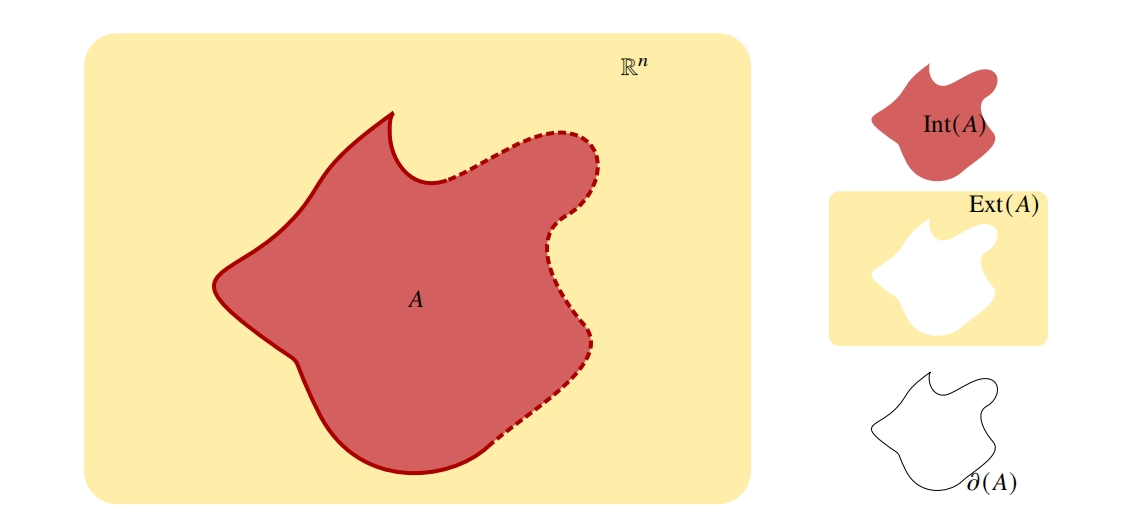
\includegraphics[width=0.6\textwidth]{figure/topological_space/int_ext_boundary.png}
    \caption{}
\end{figure}



\begin{example}{}{}
    Let $X=\{a,b,c,d,e\}$ and
    \begin{align*}
        \tau=\{X,\O,\{a\},\{c,d\},\{a,c,d\},\{b,c,d,e\}\}. 
    \end{align*} 
    Show that $\overline{\{b\}} = \{b,e\}$. 
\end{example}



\begin{definition}{}{}
    Let $A$ be a subset of a topological space $(X,\tau)$. Then $A$ is said to be dense in $X$ if $\overline{A}=X$.
    $X$ is said to be separable if there exists countable dense subset in $X$.
\end{definition}

\begin{proposition}{}{}
   Let $A$ be a subset of a topological space $(X,\tau)$. Then $A$ is dense in $X$ iff every non-empty open subset of $X$ intersects $A$ non-trivially, i.e.
   if $U\in \tau$ and $U\neq \O$ then $A\cap U\neq \O$. 
 \end{proposition}


\begin{example}{}{}
    $(X,\tau_s)$ is separable iff $X$ is countable. 
\end{example}
refer to \href{https://astarmathsandphysics.com/university-maths-notes/topology/2198-proof-that-a-discrete-space-is-separable-if-and-only-if-it-is-countable.html}{website proof}.


\begin{example}{}{}
    $(X,\tau_t)$ is separable. 
\end{example}
Let $A$ be a countably infinite subset of $X$. By example\ref{exa:limit point in trival topology}, 
$\overline{A}$ = $X$. Hence, $A$ is dense in $X$ and so $X$ is separable.
\begin{example}{}{}
    $(X,\tau_f)$ is separable.
\end{example}
    Let $A$ be a countably infinite subset of $X$. By example\ref{exa:limit point in cofinite topology}, 
    $\overline{A}$ = $X$. Hence, $A$ is dense in $X$ and so $X$ is separable.

\begin{example}{}{}
    $(X,\tau_c)$ is inseperable. 
\end{example}
    Let $A$ be a countably infinite subset of $X$.By example\ref{exa:limit point in cocountable topology},
    $\overline{A}$ = $A$. Hence, $X$ have no countably dense subset and so inseperable.

\begin{example}{}{}
    $(\R,\tau_e)$ is separable.
\end{example}
prove that $\overline{\Q}$=$\R$.


\subsection{Sequence convergence}
\begin{definition}{}{sequence convergence in topological space}
    Let $(X,\tau)$ be a topological space and $A$ a subset of $X$. Let $(x_n)_{n\in\N}$ be an infinite sequence in $A$.
    Then $(x_n)$ converages to the limit $x\in X$(denoted by $x_n\rightarrow x$) iff
    \begin{align*}
        \forall U\in \tau \text{ with }  x\in U \Rightarrow \{n\in \N:x_n\notin U\} \text{ is finite}.
    \end{align*}
    Or, 
    \begin{align*}
        \forall U\in \tau \text{ with }  x\in U \Rightarrow \exists N\in \N, \forall n>N, x_n\in U.
    \end{align*}
\end{definition}

In euclidean space,  the convergence point of a convergent sequence is unique but this is not true in cocountable space.
And in euclidean space, when $x$ is the limit point of the set $A$, there is a sequence $(x_n)$ in A, which converges to $x$. 
But this is not ture in topological space, you can recall the example\ref{exa:finit set can have limit point}, 
in which there is no sequence converges to the limit point. 
 
\begin{proposition}{}{sequence convergence in cofinite topology}
    Let $(x_n)$ be a sequence which elements are different in $(R,\tau_f)$, then $\forall x\in X$, $x_n\rightarrow x$. 
\end{proposition}
\begin{proof}
    $\forall U\in \tau \text{ with }  x\in U \Rightarrow \{n\in \N:x_n\notin U\}= \{n\in \N:x_n\in U^c\} \text{ is finite}$.
\end{proof}
\begin{proposition}{}{sequence convergence in cocountable topology}
    Let $(x_n)$ be a sequence which elements are different in $(R,\tau_f)$, then
    \begin{align*}
        x_n\rightarrow x \Leftrightarrow \exists N\in\N, \forall n>N, x_n=x. 
    \end{align*}
\end{proposition}
\begin{proof}
    ($\Leftarrow$) clear by definition\ref{def:sequence convergence in topological space}
    \\
    ($\Rightarrow$) Consider the set $B:= \{x_n: x_n\neq x\}$. Since a sequence is countable, $B$ is countable. By example\ref{exa:limit point in cocountable topology}, B is closed.
    By construction, $x\notin B$, so $U=X\setminus B$ is an open set containing $x$. 
    But $x_n\rightarrow x$, so a tail of this sequence must lie in $X\setminus B$. Since $\{x_n\}\cap (X\setminus B)=\{x\}$, 
    this means that a tail of this sequence is constanst.  
\end{proof}

\section{Subspace}
\begin{definition}{}{}
    Let $A$ be a non-empty subset of a topological space $(X\,\tau)$. 
    The collection 
    \begin{align*}
        \tau_{A}=\{O\cap A: O\in \tau\}
    \end{align*}
    of subsets of $A$ is a topology on $A$ called the subspace topology
    (or the topology induced on $A$ by $\tau$). The topological space $(A,\tau_A)$ is said to be a subspace of $(X,\tau)$.
\end{definition}
Let's check that $\tau_A$ is indeed a topology on $A$.\\
(1) $A=X\cap A, \O = \O\cap A$, then $A,\O\in \tau_A$.\\
(2) If $U_{\alpha}\in \tau_A$, then $\cup_{\alpha}{U_\alpha} = \cup_{\alpha} (O_{\alpha}\cap A)=(\cup_{\alpha} O_{\alpha})\cap A\in\tau_A$.\\
(3) If $U_1,U_2\in\tau_A$, then $U_1\cap U_2 = (O_1\cap A)\cap (O_2\cap A)=(O_1\cap O_2)\cap A\in \tau_A$.

In the following content,  we follow the convention: a subset of topological Spaces is treated as a subspace. 
\begin{proposition}{}{Subspace of Subspace is Subspace}
    Let $(X,\tau)$ be a topological space and $B\subseteq A\subseteq X$. Then $(\tau_A)_B=\tau_B$.
\end{proposition}

\begin{align*}
    (\tau_A)_B = & \{K\cap B:K\in \tau_A\} \\
        =  &\{(O\cap A)\cap B: O\in\tau\} \\
        =  &\{(O\cap B)\cap (A\cap B): O\in \tau\}\\
        \overset{B\subseteq A}{=}  &\{(O\cap B)\cap B: O\in \tau\}\\
        =  &\{(O\cap B): O\in \tau\}\\
        =  &\tau_B.
\end{align*}
Hence, there are two way to induce the topology on $B$: induced by the topology on $A$ or
induced by the topology on $X$.

\begin{example}{}{}
    Let $X=\{a,b,c,d,e,f\}$, 
    \begin{align*}
        \tau = \{X,\O, \{a\}, \{c,d\}, \{a,c,d\}, \{b,c,d,e,f\}\},
    \end{align*}
    and $A=\{b,c,e\}$. Then the subspace topology on $A$ is 
    \begin{align*}
        \tau_A = \{A,\O, \{c\}\}.
    \end{align*}
\end{example}


Consider the subset $[1,2]$ of $(\R,\tau_e)$. Then the topology on $[1,2]$ is 
\begin{align*}
    \tau = \{(a,b)\cap [1,2]: (a,b)\in \tau_e\}.
\end{align*}
\par
But here we see some surprising things happening; e.g.
$[1,\frac{3}{2})$ is certainly not an open set in $\R$, but $[1,\frac{3}{2})=(1,\frac{3}{2})\cap [1,2]$, is an open set in the subspace $[1,2]$.
\par
Also $(1,2]$ is not open in $\R$ but is open in $[1,2]$. Even $[1,2]$ is not open in $\R$, but is an open set in $[1,2]$.
\par
So whenever we speak of a set being open we must make perfectly clear in what space or what topology it is an open set. 

\begin{proposition}{}{closed in subspace}
    Let $(X,\tau)$ be a topological space and $C\subset A\subset X$, then
    \begin{align*}
        C \text{ is closed in } A\Leftrightarrow C = A\cap V, \text{ where $V$ is closed in $X$}.  
    \end{align*}
\end{proposition}
\begin{proof}
    % \begin{align*}
    %     C \text{ is closed in } A &\Leftrightarrow A\setminus C \text{ is open in } A &\\
    %     & \Leftrightarrow \exists O\in \tau_{X}, \text{ s.t. } A\setminus C = O\cap A &\\
    %     & \Leftrightarrow \exists O\in \tau_{X}, C && = A\setminus(O\cap A) = (A\setminus O) \cup (A\setminus A) = &\\
    %     & &(A\setminus O) \cup \O = A\setminus O\\
         
    % \end{align*}

    \begin{align*}
        C \text{ is closed in } A &\Leftrightarrow A\setminus C \text{ is open in } A\\
         &\Leftrightarrow \exists O\in \tau_{X}, \text{ s.t. } A\setminus C = O\cap A\\
         &\Leftrightarrow \exists O\in \tau_{X}, C= A\setminus(O\cap A) \\
         &\quad\quad = (A\setminus O) \cup (A\setminus A)\\
         &\quad\quad = (A\setminus O) \cup \O = A\setminus O\\
         &\quad\quad = (A\cap X)\setminus O\\
         &\quad\quad = A\cap (X\setminus O)\\
         &\quad\quad = A\cap V, \text{ where $V$ is closed in $X$.}
        \end{align*}
\end{proof}

\begin{proposition}{}{closed transitive1}
    Let $(X,\tau)$ be a topological space, $B\subset A\subset X$, then\\
    (1) If $B$ is open(closed) in $X$, then $B$ is open(closed) in $A$;\\
    (2) If $A$ is open(closed) in $X$ and $B$ is open(closed) in $A$, then $B$ is open(closed) in $X$.
\end{proposition}
\begin{proof}
    (1) We know that $B=B\cap A$. If $B=O$ , then $B = O\cap A$ and so $B$ is open in $A$. 
    If $B$ is closed in $X$, by proposition\ref{prop:closed intersection}, $B=X\cap V$, where $V$ is closed in $X$. 
    Then $B=B\cap A = (X\cap V)\cap A = (X\cap A)\cap V$, by by proposition\ref{prop:closed intersection}, $B$ is closed in $A$.\\
    (2) If $B = O_1\cap A$ and $A=O_2$ , then $B=O_1\cap O_2\in \tau$ and so $B$ is open in $X$.
    If $A$ is closed in $X$ and $B$ is closed in $A$, then $A = X\cap V_1, B=A\cap V_2$, where $V_1,V_2$ is closed in $X$.
    Then, $B = X\cap (V_1\cap V_2)$. As $V_1\cap V_2$ is closed in $X$, $B$ is closed in $X$. 
\end{proof}

\begin{corollary}{}{closed transitive2}
    Let subspace $A$ be closed in $X$. Then 
    $C\subset A$ is closed in $A$ iff $C$ is closed in $X$.
\end{corollary}
\begin{proof}
    ($\Rightarrow$): By proposition\ref{prop:closed in subspace}, $\exists V$ which is closed in $X$ such that $C=A\cap V$.
    Since $A$ and $V$ are closed in $X$, it follows that $C=A\cap V$ is closed in $X$.
    \\
    ($\Leftarrow$): By proposition\ref{prop:closed transitive1}.
\end{proof}

\begin{proposition}{}{}
    Let $(X,\tau)$ be a topological space and $A\subset Y\subset X$. Then $\text{cl}_Y(A)=A\cap \text{cl}_X(A)$.
\end{proposition}

\begin{proof}
    $\text{cl}_Y=\cap \{K\subseteq Y:A\subseteq K, k \text{ is closed in} Y\}$\\
    
\end{proof}

\section{Reference}
\begin{itemize}
    \item \href{https://www.ms.uky.edu/~guillou/F14/551Notes-Week4.pdf}{lecture notes from uky}
    \item \href{http://staff.ustc.edu.cn/~wangzuoq/Courses/21S-Topology/Notes/Lec07.pdf}{lecture notes from ustc}
\end{itemize}
\section{Exercise}

